% Отчёт к курсовой работе (алгоритм Прима).
% Компиляция: xelatex report.tex (дважды — для оглавления).
\documentclass[a4paper,14pt]{extarticle}

\usepackage{fontspec}
\setmainfont{Times New Roman}
\setmonofont{Consolas}
\emergencystretch=3em

\usepackage{polyglossia}
\setdefaultlanguage{russian}
\setotherlanguage{english}

\usepackage[left=3cm,right=1.5cm,top=2cm,bottom=2cm]{geometry}
\usepackage{amsmath}
\usepackage{graphicx}
\usepackage{listings}
\usepackage{xcolor}
\usepackage{caption}
\usepackage{setspace}

\onehalfspacing

\usepackage[hidelinks]{hyperref}

% --- Данные титульного листа (заполнить) ---
\newcommand{\StudentName}{Фамилия И. О.}
\newcommand{\StudentGroup}{Группа}
\newcommand{\TeacherName}{Фамилия И. О. преподавателя}
\newcommand{\CourseYear}{2026}

% --- Стиль листингов ---
\renewcommand{\lstlistingname}{Листинг}
\lstset{
  basicstyle=\ttfamily\small,
  breaklines=true,
  frame=single,
  numbers=left,
  numberstyle=\tiny\color{gray},
  xleftmargin=1.5em,
  framexleftmargin=1em,
  showstringspaces=false,
  keywordstyle=\color{blue},
  commentstyle=\color{gray},
  stringstyle=\color{teal},
}

\captionsetup{labelsep=endash}

\begin{document}

% ================= Титульный лист =================
\begin{titlepage}
  \centering
  {\small МИНИСТЕРСТВО НАУКИ И ВЫСШЕГО ОБРАЗОВАНИЯ РОССИЙСКОЙ ФЕДЕРАЦИИ\par}
  \vspace{0.4cm}
  {\small ФЕДЕРАЛЬНОЕ ГОСУДАРСТВЕННОЕ АВТОНОМНОЕ ОБРАЗОВАТЕЛЬНОЕ УЧРЕЖДЕНИЕ ВЫСШЕГО ОБРАЗОВАНИЯ\par}
  \vspace{0.4cm}
  {\small «САНКТ-ПЕТЕРБУРГСКИЙ ГОСУДАРСТВЕННЫЙ УНИВЕРСИТЕТ АЭРОКОСМИЧЕСКОГО ПРИБОРОСТРОЕНИЯ»\par}

  \vspace{3cm}
  {\large КУРСОВАЯ РАБОТА\par}
  \vspace{0.6cm}
  {\large по дисциплине «Программирование»\par}
  \vspace{0.8cm}
  {\Large Тема: «Алгоритм Прима: построение минимального остовного дерева»\par}

  \vfill
  \begin{flushright}
    \begin{tabular}{l}
      Выполнил: студент группы \StudentGroup \\[0.2cm]
      \StudentName \\[0.6cm]
      Проверил: \TeacherName \\
    \end{tabular}
  \end{flushright}

  \vspace{1.5cm}
  {\small Санкт-Петербург\par}
  {\small \CourseYear\par}
\end{titlepage}

% ================= Оглавление =================
\tableofcontents
\newpage

% ================= 1. Постановка задачи =================
\section{Постановка задачи}

Задачей данной курсовой работы является разработка программы, которая по
заданному взвешенному неориентированному связному графу строит его
минимальное остовное дерево с помощью алгоритма Прима и сохраняет полученный
результат в текстовый файл в формате graphviz (DOT).

Пусть задан связный неориентированный граф $G=(V,E)$, каждому ребру
$e \in E$ которого приписан неотрицательный вес $w(e)$. Остовным деревом
(каркасом) графа называется такой его подграф $T=(V,E')$, который содержит
все вершины исходного графа и при этом является деревом, то есть связным
графом без циклов. Минимальным остовным деревом называется остовное дерево,
сумма весов рёбер которого минимальна среди всех остовных деревьев данного
графа. Если в графе имеются рёбра одинакового веса, минимальное остовное
дерево может быть не единственным; в этом случае программа выводит одно из
возможных.

Задача имеет практический смысл: минимальное остовное дерево описывает,
например, наиболее дешёвый способ соединения нескольких объектов сетью
(дорогами, линиями связи, трубопроводами) без образования циклов. Связность
дерева гарантирует достижимость любого объекта, а отсутствие циклов ---
отсутствие избыточных соединений.

Осмысленность задачи можно показать на примере. Для графа, изображённого на
рисунке~\ref{fig:graph}, существуют остовные деревья различной стоимости.
Так, дерево, состоящее из рёбер $(0,1)$, $(1,2)$, $(1,3)$, $(3,4)$ и $(4,5)$,
имеет суммарный вес $4+1+5+2+3=15$, тогда как дерево из рёбер $(0,2)$,
$(1,2)$, $(1,3)$, $(3,4)$ и $(4,5)$ имеет вес $2+1+5+2+3=13$. Таким образом,
выбор дерева минимальной стоимости не является тривиальным. Подробное
описание задачи и алгоритма её решения приведено в книге [1].

% ================= 2. Алгоритм =================
\section{Алгоритм}

\subsection{Идея алгоритма}

Алгоритм Прима относится к классу жадных алгоритмов. Он строит минимальное
остовное дерево постепенно: на каждом шаге к уже построенной части дерева
присоединяется ребро минимального веса, один конец которого лежит в дереве,
а другой --- вне его. Построение начинается с произвольной вершины (в данной
реализации --- с вершины с номером 0). Процесс продолжается до тех пор, пока в
дерево не будут включены все вершины графа.

\subsection{Структуры данных}

В программе используются следующие структуры данных:
\begin{itemize}
  \item граф хранится в виде списков смежности --- контейнера
        \texttt{std::vector<std::vector<Edge>>}, где \texttt{Edge} ---
        структура, содержащая номера вершин и вес ребра;
  \item множество вершин, уже включённых в дерево, представляется булевым
        вектором \texttt{std::vector<bool>};
  \item для выбора ребра минимального веса, пересекающего разрез (множество
        рёбер, соединяющих вершины дерева с остальными вершинами),
        используется очередь с приоритетом \texttt{std::priority\_queue},
        основанная на двоичной куче.
\end{itemize}

\subsection{Пошаговое выполнение на примере}

Рассмотрим работу алгоритма на графе, изображённом на
рисунке~\ref{fig:graph}. Построение начинается с вершины 0.

\begin{enumerate}
  \item Дерево состоит из вершины $\{0\}$. Рёбра, пересекающие разрез:
        $(0,1)$ с весом 4 и $(0,2)$ с весом 2. Выбирается ребро минимального
        веса $(0,2)$; вершина 2 включается в дерево.
  \item Дерево: $\{0,2\}$. Рёбра, пересекающие разрез: $(0,1)$, $(1,2)$,
        $(2,3)$, $(2,4)$. Минимальное --- $(1,2)$ с весом 1; вершина 1
        включается в дерево.
  \item Дерево: $\{0,1,2\}$. Из рёбер $(2,3)$, $(2,4)$, $(1,3)$ выбирается
        $(1,3)$ с весом 5; вершина 3 включается в дерево.
  \item Дерево: $\{0,1,2,3\}$. Из рёбер $(2,4)$, $(3,4)$, $(3,5)$ выбирается
        $(3,4)$ с весом 2; вершина 4 включается в дерево.
  \item Дерево: $\{0,1,2,3,4\}$. Из рёбер $(3,5)$, $(4,5)$ выбирается $(4,5)$
        с весом 3; вершина 5 включается в дерево.
\end{enumerate}

Все вершины включены в дерево; построение завершено. Суммарный вес
минимального остовного дерева равен $2+1+5+2+3=13$. Результат приведён на
рисунке~\ref{fig:mst}.

\subsection{Псевдокод}

\begin{lstlisting}[caption={Псевдокод алгоритма Прима},label=lst:prim]
АЛГОРИТМ Прима(G, start = 0):
    in_tree[v] <- false для всех v из V
    tree_edges <- пустой список рёбер
    total_weight <- 0

    in_tree[start] <- true
    frontier <- пустая очередь с приоритетом (минимум по весу)
    для каждого ребра e = (start, u, w) из G.adjacency(start):
        frontier.push((w, e))

    пока frontier не пуста:
        (w, e) <- frontier.top(); frontier.pop()
        если in_tree[e.to] == true:
            continue    // ребро ведёт в уже включённую вершину
        in_tree[e.to] <- true
        tree_edges.push_back(e)
        total_weight <- total_weight + w
        для каждого ребра next = (e.to, x, w2) из G.adjacency(e.to):
            если in_tree[x] == false:
                frontier.push((w2, next))

    вернуть (tree_edges, total_weight)
\end{lstlisting}

\subsection{Анализ сложности}

Каждая вершина включается в дерево ровно один раз, поэтому цикл построения
дерева выполняется не более $|V|$ раз. Каждое ребро графа попадает в очередь
с приоритетом не более двух раз (по одному разу для каждого из своих концов),
поэтому общее количество операций с кучей не превосходит $2|E|$. Операции
вставки и извлечения минимума из двоичной кучи выполняются за $O(\log n)$, где
$n$ --- количество элементов в куче, не превосходящее $|E|$. Таким образом,
временная сложность алгоритма составляет $O((V+E)\log E)$. Поскольку в
простом графе $|E| \le |V|(|V|-1)/2$, справедливо $\log E = O(\log V)$,
поэтому сложность можно записать как $O((V+E)\log V)$. Затраты памяти
составляют $O(V+E)$.

% ================= 3. Инструкция пользователя =================
\section{Инструкция пользователя}

\subsection{Запуск программы}

Программа запускается из командной строки и принимает два аргумента --- имена
входного и выходного файлов:

\begin{lstlisting}[language=bash]
prim.exe input.txt output.dot
\end{lstlisting}

\subsection{Формат входного файла}

Входной файл содержит матрицу смежности весов графа. В первой строке задано
количество вершин $N$, далее следуют $N$ строк по $N$ чисел. Число $0$
означает отсутствие ребра, положительное число --- вес ребра. Граф
неориентированный, поэтому матрица должна быть симметричной.

\subsection{Формат выходного файла}

Выходной файл содержит граф в формате DOT, поддерживаемом программой graphviz.
В файл записываются все вершины графа и рёбра построенного минимального
остовного дерева с указанием весов; суммарный вес дерева указывается в
подписи графа. Такой файл можно преобразовать в изображение командой
\texttt{dot -Tpng output.dot -o graph.png}.

% ================= 4. Тестовые примеры =================
\section{Тестовые примеры}

Ниже приведены три тестовых примера. Для каждого указаны входной файл,
полученный выходной файл и суммарный вес минимального остовного дерева.

\subsection{Тест 1. Четыре вершины}

Входной файл:
\begin{lstlisting}
4
0 1 2 3
1 0 4 5
2 4 0 6
3 5 6 0
\end{lstlisting}

Выходной файл:
\begin{lstlisting}
graph MST {
    label = "Minimum spanning tree (Prim's algorithm), total weight = 6";
    node [shape = circle];
    0; 1; 2; 3;
    0 -- 1 [label = "1"];
    0 -- 2 [label = "2"];
    0 -- 3 [label = "3"];
}
\end{lstlisting}

Суммарный вес: $6$.

\subsection{Тест 2. Пять вершин}

Входной файл:
\begin{lstlisting}
5
0 2 0 6 0
2 0 3 8 5
0 3 0 0 7
6 8 0 0 9
0 5 7 9 0
\end{lstlisting}

Выходной файл:
\begin{lstlisting}
graph MST {
    label = "Minimum spanning tree (Prim's algorithm), total weight = 16";
    node [shape = circle];
    0; 1; 2; 3; 4;
    0 -- 1 [label = "2"];
    1 -- 2 [label = "3"];
    1 -- 4 [label = "5"];
    0 -- 3 [label = "6"];
}
\end{lstlisting}

Суммарный вес: $16$.

\subsection{Тест 3. Шесть вершин}

Входной файл:
\begin{lstlisting}
6
0 4 2 0 0 0
4 0 1 5 0 0
2 1 0 8 10 0
0 5 8 0 2 6
0 0 10 2 0 3
0 0 0 6 3 0
\end{lstlisting}

Выходной файл:
\begin{lstlisting}
graph MST {
    label = "Minimum spanning tree (Prim's algorithm), total weight = 13";
    node [shape = circle];
    0; 1; 2; 3; 4; 5;
    0 -- 2 [label = "2"];
    2 -- 1 [label = "1"];
    1 -- 3 [label = "5"];
    3 -- 4 [label = "2"];
    4 -- 5 [label = "3"];
}
\end{lstlisting}

Суммарный вес: $13$.

% ================= Рисунки =================
\begin{figure}[h!]
  \centering
  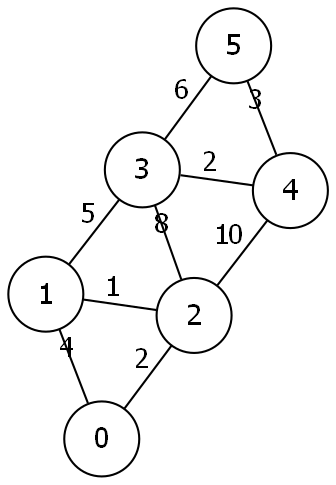
\includegraphics[width=0.65\textwidth]{fig/fig_graph.png}
  \caption{Исходный взвешенный неориентированный граф}
  \label{fig:graph}
\end{figure}

\begin{figure}[h!]
  \centering
  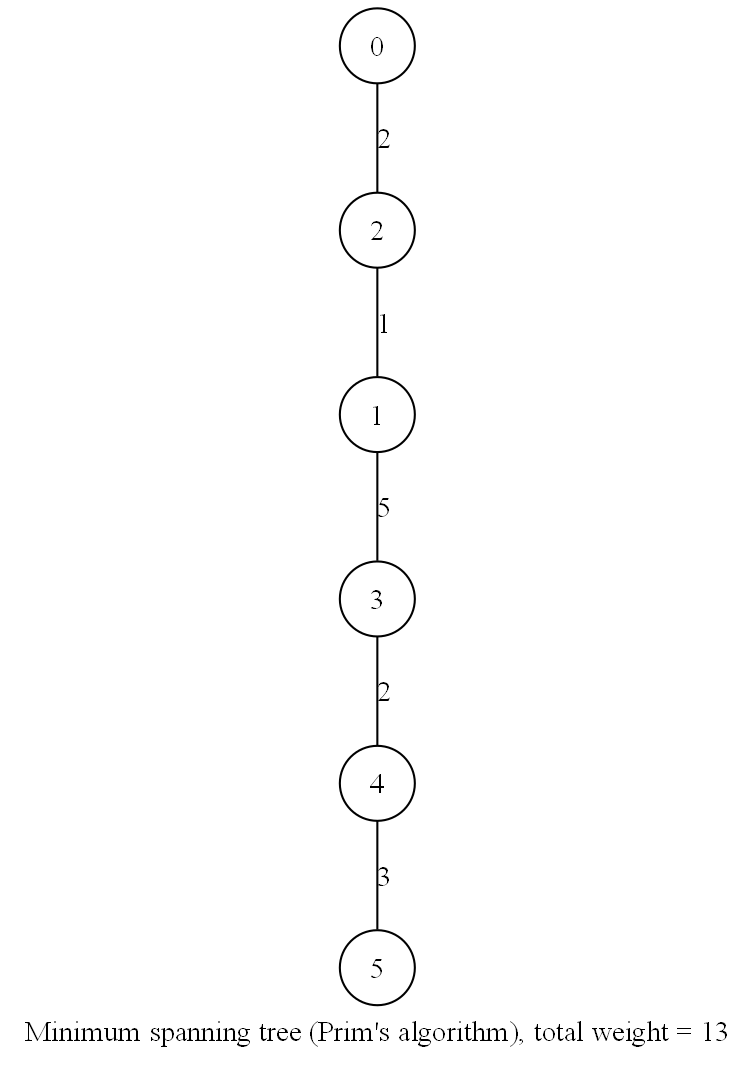
\includegraphics[width=0.6\textwidth]{fig/fig_mst.png}
  \caption{Минимальное остовное дерево --- результат работы программы,
           отрисованный программой graphviz}
  \label{fig:mst}
\end{figure}

% ================= Список литературы =================
\begin{thebibliography}{9}
  \bibitem{aho} Ахо А., Хопкрофт Дж., Ульман Дж. Построение и анализ
  вычислительных алгоритмов. --- М.: Мир, 1979.
  \bibitem{cormen} Кормен Т., Лейзерсон Ч., Ривест Р., Штайн К. Алгоритмы:
  построение и анализ. --- 3-е изд. --- М.: Вильямс, 2013.
  \bibitem{graphviz} Graphviz --- Graph Visualization Software [Электронный
  ресурс]. --- URL: \url{https://graphviz.org/} (дата обращения: 2026).
\end{thebibliography}

% ================= Приложение. Листинг исходного кода =================
\section*{Приложение. Листинг исходного кода}
\addcontentsline{toc}{section}{Приложение. Листинг исходного кода}

\lstinputlisting[language=C++, caption={Файл src/main.cpp}, label=lst:main]{../src/main.cpp}
\lstinputlisting[language=C++, caption={Файл inc/graph.h}, label=lst:graphh]{../inc/graph.h}
\lstinputlisting[language=C++, caption={Файл src/graph.cpp}, label=lst:graphcpp]{../src/graph.cpp}
\lstinputlisting[language=C++, caption={Файл inc/prim.h}, label=lst:primh]{../inc/prim.h}
\lstinputlisting[language=C++, caption={Файл src/prim.cpp}, label=lst:primcpp]{../src/prim.cpp}

\end{document}
